\chapter{Backgrounds}
\label{chap:backgrounds}

\section{Hardware Design Paradigms}
\label{sec:design-paradigm}

Traditional Register-Transfer Level (RTL) designs require hardware
designers to consider scheduling for all resources. During hardware
design, it is required that any resource elements are correctly
employed, e.g., one should not write a register more than once in the
same cycle, which would cause an uncertain behavior. If a particular
input port of a hardware component is used more than once, we do not
have any guarantees for the output value, also causing an uncertain
use of values. A well-known RTL design framework,
Verilog~\cite{verilog}, lets users take responsibility for this, thus
they should carefully investigate if there is an assignment which
makes an uncertain state transition.
\begin{figure}[h]
  \centering
  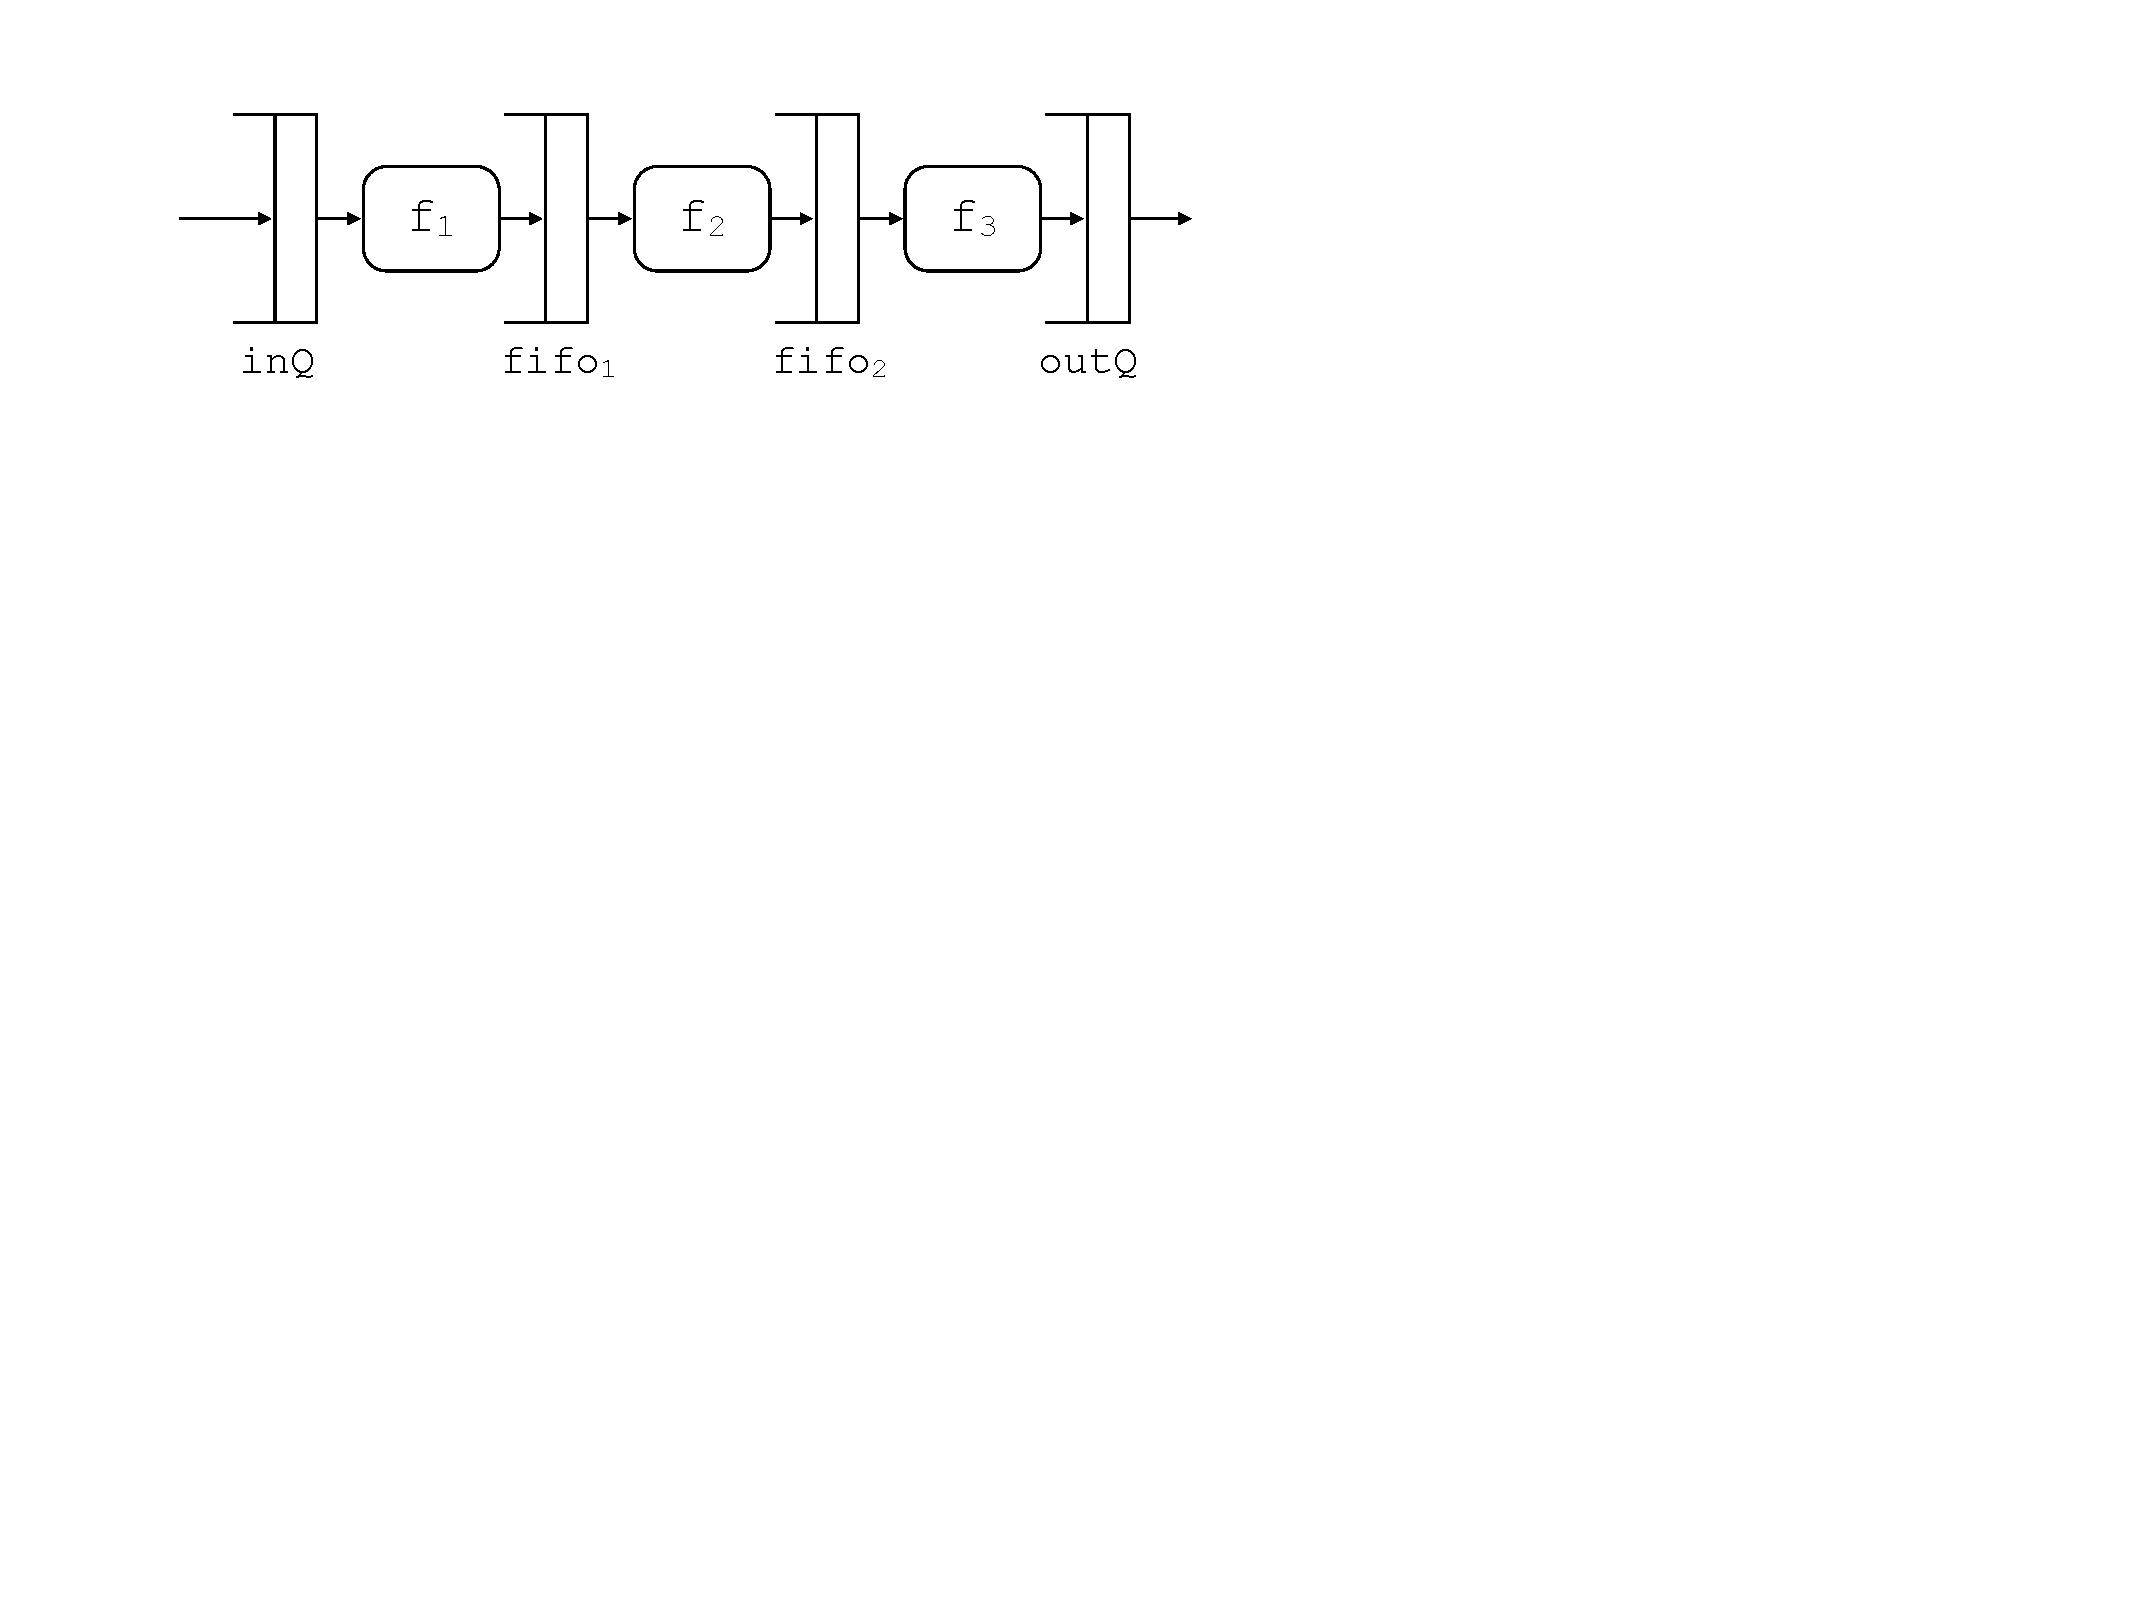
\includegraphics[width=0.5\textwidth]{figures/pipeline.pdf}
  \caption{A pipelined system}
  \label{fig-pipelined-system}
\end{figure}

A disadvantage of this approach is that having no separation between
functional parts and scheduling logic makes maintenance harder. Let us
revisit the pipelined system where three systems $f_1$, $f_2$, and
$f_3$ are connected by fifos, as shown in
\reffig{fig-pipelined-system}. For simplicity, suppose that only one
element can reside in a fifo. Since there is only one element in a
fifo, push and pop cannot be requested in the same cycle, since it
causes a double-write. Now the problem occurs because we have no
information whether push and pop will be requested simultaneously or
not. Thus in this case, we cannot avoid an implementation tightly
coupled with scheduling logic; for each case of push and pop, there is
no way for user except to define control flags for push and pop.

For this reason, in some frameworks like Verilog, designers tend to
specify the data path first, and then to define the controlling logic
which is entangled with the data path design. The problem with this
conventional design approach is that it is not flexible in perspective
of verification. If a designer specifies the controlling logic clearly
for a hardware system, it would be easy to verify it. However, since
the specification is only for the parcicular hardware system, the
verification approach used for the system may not be reusable for
other systems, even if they have similar designs.

Guarded Atomic Action (GAA) is a design paradigm used by \Bluespec{}
for correct and effective scheduling that makes up for shortcomings of
the RTL designs. It is different from the traditional RTL designs
mentioned above. The main idea is that any hardware system has a
(structural) state component that can be captured by a set of
variables that represent registers or storage. State transition is
done by a set of rules, where a rule is a series of actions with
\emph{guards} on this state. A guard of a rule is a predicate that
should be satisfied to execute the rule. Each action (including one
for rules) should be atomic -- an execution of an action should be
guaranteed to make a state transition purely caused by the action.

\section{Semantics of the Bluespec Language}
\label{sec:bluespec-semantics}

\paragraph{Module structure}

Modularity forms the base semantics of the \Bluespec{} language. It is
simply to follow a natural hardware design concept. Designers usually
develop complex hardware components in a modular manner; small module
components are designed first, and they are composed to build a large
and complex one.

Bluespec supports such module definitions. Each module has a set of
registers, called an \emph{internal state} of the module. The internal
state can be modified only by the module itself. In order to induce a
state change from the outside of the module, it should be requested by
method calls. The module also has a set of \emph{rules}. Each rule is
composed of GAAs. Rules are executed by a global rule scheduler. The
scheduler selects the maximal number of rules where the guards of the
rules do not conflict each others. Once the scheduler confirms the
validity of the guards, they are executed concurrently. Lastly, the
module has a set of \emph{methods}. Bluespec separates the notion of
\emph{Method} and \emph{ActionMethod}. Method is like a macro, which
evaluates an expression. From the perspective of hardware, Method can
be synthesized to a combinational circuit.  Whereas, ActionMethod is
composed of GAAs, which only can be called by external modules. Thus,
it acts like an interface of the module. ActionMethod is the only way
to manipulate internal states from outside.

\begin{figure}[t]
  \centering{
    \begin{subfigure}[b]{0.5\textwidth}
      \bsvmodinst{PipelinedSystem}{inQ, fifo1, fifo2, outQ}{
        \bsvnone{\pgmrule}{stage0}{}{
          \pgmif{} \textrm{inQ.empty \&\& fifo1.notFull} \\
          \pgmthen{} \textrm{fifo1.enq(f0(inQ.first)); inQ.deq;}
        }\\
        \bsvnone{\pgmrule}{stage1}{}{
          \pgmif{} \textrm{fifo1.notEmpty \&\& fifo2.notFull} \\
          \pgmthen{} \textrm{fifo2.enq(f1(fifo1.first)); fifo1.deq;}
        }\\
        \bsvnone{\pgmrule}{stage2}{}{
          \pgmif{} \textrm{fifo2.notEmpty \&\& outQ.notFull} \\
          \pgmthen{} \textrm{outQ.enq(f2(fifo2.first)); fifo2.deq;}
        }\\
        \bsvnone{\pgmameth}{req}{(x)}{
          \textrm{inQ.enq(x);}
        }\\
        \bsvnone{\pgmameth}{res}{}{
          \pgmletin{x}{outQ.first}
          \textrm{outQ.deq;} \\
          \pgmret{x}
        }
      }
    \end{subfigure}
  }
  \caption{The pipelined system implemented with Bluespec}
  \label{ex-pipelined-system-bluespec}
\end{figure}

\reffig{ex-pipelined-system-bluespec} describes the psuedo-code
Bluespec module definition of the pipelined system presented in
\reffig{fig-pipelined-system}. The big module PipelinedSystem has four
module instances, named inQ, fifo1, fifo2, and outQ. It has three
rules (stage0, stage1, and stage2); each rule pulls an element from a
fifo, applies an operation, and push the resulting value to the next
fifo. The module has two interface methods: ``req'' is called when
there is a request with argument ``x'', and ``res'' is called to get
the result value.

\paragraph{Well-formedness of a module}

Syntactic correctness of a module does not imply a correct
execution. In other words, the module should satisfy an additional
number of conditions in order for valid execution. Firstly, a rule or
a method should not perform a write operation to the same register
twice (double-write). It also should not call the same method twice
(double-call). This is simply because actions in a rule (a method) are
executed simultaneously. A second condition is that method calls
cannot form a cycle among modules, since the cycle has no valid
behaviors in terms of hardware design. The last condition is that
register reads and writes should be defined within the module in which
the register is defined.

These conditions are sometimes called a well-formedness of a
module. It is usually defined independently with semantics, since it
can be captured statically by traversing the module definition. We
formally define the well-formedness on \refsect{sec-wf}, and use it on
the correctness proof of an inlining operation. See the section for
more details.

\paragraph{Concurrent rule executions}

A guard of a rule includes facts that which registers are written and
which methods are called. Since the guard contains conditions to
execute the rule, it is natural for the guard to have conditions for
register writes and method calls. If there are no explicit guard
conditions on the definition of a rule, then the guard only consists
of register and method conditions. Guards contain such conditions in
order to ensure that there are no double-writes or double-calls during
multiple rule executions. Even if they are caught by forcing the
well-formedness condition, it is restricted within a rule or a
method. We cannot statically ensure if multiple rules can be executed
concurrently, without violating double-writes and double-calls.

Based on guards of rules, a rule scheduler tries to find a maximal set
of guards for the rules to be executed concurrently. The guards of
concurrently executed rules do not conflict each other. For instance,
all the rules of PipelinedSystem can be executed concurrently. In
other words, the rule scheduler can verify that the guards of the
three rules in PipelinedSystem do not conflict. This is because the
rules do not write the same register and do not call the same method.

\paragraph{One-rule-at-a-time semantics}

Multiple rule executions require an additional condition other than
non-conflicting guards, which is called the one-rule-at-a-time
semantics. The condition says that, multiple rules can be executed if
there \emph{exists a permutation of the rules} which yields the same
state change if they are executed sequentially. More formally, when we
define $(r_1; r_2; \cdots; r_n)$ be the concurrent execution of the
rules, then there exists $\{r_{p_1}, r_{p_2}, \cdots, r_{p_n}\}$, a
permutation of the rules, such that
\begin{center}
  \begin{math}
    \forall s. (r_1; r_2; \cdots; r_n)(s) = r_{p_n}(\cdots(r_{p_2}(r_{p_1}(s)))\cdots),
  \end{math}
\end{center}
where $s$ is an internal state of the module.

One-rule-at-a-time semantics makes verification easier. As the name
indicates, it is fine to consider semantics where at most one rule is
executed at a time. Once we verify some properties under the
one-rule-at-a-time semantics, the whole system, in which a rule
scheduler is attached, also can be verified simply by proving that the
scheduler always selects rules based on the one-rule-at-a-time
semantics.

\section{Previous Semantic Designs}
\label{sec:related-works}

\paragraph{Operational semantics}

An operational big-step semantics for a Bluespec-like language has
been defined~\cite{nirav-memocode}, but not for verification. The
semantics was defined for explaining how multiple rules are executed
by a rule scheduler, using the notion of rule composition. The target
language is BTRS, a Bluespec program after type checking and module
instantiations. BTRS is defined in order to make the language and the
rule scheduling algorithm deterministic. However, no formal proofs are
presented for the correctness of the rule scheduling algorithm by
using the semantics. Furthermore, the semantics is only defined for
\emph{closed systems}, not for \emph{open systems}. A closed system
implies that all methods which are called are explicitly defined
somewhere. In contrast, an open system allows method calls where the
methods are not defined yet. When a semantics is defined only for
closed systems, it is not suitable for scalable verification since it
always requires a fully defined system.

The formal semantics for open hardware system has been subsequently
defined based on modularity~\cite{murali-thesis}. The core concept for
the semantics is modularity; it defines behaviors of small basic
modules, and combines them in order to define behaviors of a big
module composed of the small ones. For such modular designs, the
semantics should be able to describe behaviors of open systems, since
small modules may call methods outside of them. The modular semantics
has been formally defined and used in the \Kami{} framework, described
by the Coq proof assistant.

However, the modular semantics has an inherent weakness that it is
hard to infer the internal state changes only by looking at external
communications.
\begin{figure}[t]
  \centering{
    \begin{subfigure}[b]{0.5\textwidth}
      \bsvmodnoreg{m}{
        \bsvnone{\pgmrule}{s}{}{
          \pgmwrite{r_1}{1}
          \pgmcalln{f}{}
        }\\
        \bsvnone{\pgmmeth}{f}{()}{
          \pgmwrite{r_2}{2}
          \pgmcalln{g}{}
        }\\
        \bsvnone{\pgmmeth}{g}{()}{
          \pgmwrite{r_3}{3}
          \pgmcalln{h}{}
        }
      }
    \end{subfigure}
  }
  \caption{Tracking internal state changes by internal calls}
  \label{ex-modular-semantics-disadvantage}
\end{figure}
\reffig{ex-modular-semantics-disadvantage} describes the case where we
have a difficulty to infer internal state changes. Suppose a rule $s$
is executed in a module $m$. In the modular semantics, $m$ is
\emph{abstracted} so that we cannot see the actual bodies of rules or
methods. In this situation, when having information that $s$ is
executed and $h$ is externally called, how do we draw the state
changes in the module $m$? Since the modular semantics is abstracted,
it is hard to draw the internal information.

The two semantics have trade-offs. The big-step
semantics~\cite{nirav-memocode} does not have such a weakness, since
it simply traverses action bodies to draw state changes in a big-step
manner. However, as mentioned, it is not defined for open systems. On
the other hand, the modular semantics can describe open system
behaviors, but it has a weakness mentioned above. The main
contribution of this thesis is to develop a new semantic definition
which maintains modularity concept but resolves the weakness.

\paragraph{Inlining}

The basic idea of the new semantic definition is to take advantage of
a static inlining operation. We maintain the modular semantics, and
use the inlining to concretize all internal communications by
substituting method calls to their action bodies. The detailed
inlining operation is defined on \refsect{sec:inlining-semantics}.

Static inlining is not a new idea in Bluespec. It has been defined for
merging rules and methods~\cite{daniel-thesis}. It was used to convert
between two Bluespec-like languages, where one has a module hierarchy,
while the other does not have the hierarchy. The purpose of the use of
inlining is similar in that it \emph{flattens} modules to analyze them
efficiently. However, the inlining operation defined in this thesis is
more complicated in that it is defined for open systems. In other
words, the inlining does not affect communications with external
modules. Detailed proofs (called the correctness of the inlining
operation) is described in \refchap{chap:implication}.


